%% ============================================================================
%% pyhydra: an open, modular Python library for reproducible hydroclimatic
%% modelling and probabilistic flood-risk analysis
%% Target journal: SoftwareX (Elsevier) -- Original Software Publication (OSP)
%% Prepared against SoftwareX article template v6 (March 2026)
%% ============================================================================
\documentclass[preprint,12pt,a4paper]{elsarticle}

\usepackage{amsmath,amssymb}
\usepackage{booktabs}
\usepackage{array}
\usepackage{graphicx}
\usepackage{xcolor}
\usepackage[section]{placeins}
\usepackage{listings}
\usepackage{hyperref}
\usepackage{cleveref}
\hypersetup{hidelinks}

\setlength{\parindent}{0pt}

\definecolor{codebg}{HTML}{F4F6F7}
\lstset{
  basicstyle=\ttfamily\footnotesize,
  backgroundcolor=\color{codebg},
  columns=fullflexible,
  breaklines=true,
  frame=single,
  framesep=4pt,
  xleftmargin=4pt,
  xrightmargin=4pt,
  language=Python,
  showstringspaces=false,
  keywordstyle=\color{blue!60!black},
  commentstyle=\color{gray!60!black}\itshape
}

\journal{SoftwareX}
\biboptions{numbers,sort&compress}

\begin{document}

\begin{frontmatter}

\title{pyhydra: an open, modular Python library for reproducible hydroclimatic modelling and probabilistic flood-risk analysis}

\author[1]{Salvador Navas\corref{cor1}}
\ead{salvador.navas@alumnos.unican.es}
\ead[url]{https://orcid.org/0000-0001-7439-1743}
\cortext[cor1]{Corresponding author.}

\affiliation[1]{organization={IHCantabria -- Instituto de Hidr\'aulica Ambiental de la Universidad de Cantabria},
                addressline={Calle Isabel Torres 15, PCTCAN},
                city={Santander},
                postcode={39011},
                state={Cantabria},
                country={Spain}}

\author[2]{Manuel del Jesus}
\ead[url]{https://orcid.org/0000-0003-0703-8960}

\affiliation[2]{organization={Departamento de Ciencias y T\'ecnicas del Agua y del Medio Ambiente, Universidad de Cantabria},
                addressline={Avenida de los Castros 44},
                city={Santander},
                postcode={39005},
                state={Cantabria},
                country={Spain}}

\begin{abstract}
Flood-risk studies typically chain data acquisition, extreme-value and
dependence statistics, stochastic scenario generation, climate bias
correction and hydrological/hydraulic simulation through ad-hoc,
difficult-to-reuse scripts, which hampers reproducibility and transfer
between catchments, teams and regulatory contexts. \textbf{pyhydra} is an
open, modular Python library that consolidates this chain into a single
installable scientific core, organised in fifteen sub-modules: harmonised
access to hydro-climatic and hydrological data from public services,
extreme-value and copula-based statistics, stochastic rainfall generation,
climate bias correction, hybrid statistical--dynamical downscaling,
automation of HEC-HMS, HEC-RAS, SFINCS and SWAT+, propagation of
uncertainty through Monte Carlo ensembles, bootstrap confidence intervals
and Bayesian inference, and a pilot-based rule that decides, within a fixed
simulation budget, whether an expensive solver's response can be emulated
or should instead be sampled by direct Monte Carlo. Individual modules can be used independently once
the core package is installed via \texttt{pip} from its GitHub repository
(not yet on PyPI); a companion platform, HYDRA, optionally exposes the same
notebooks through a browser-based Docker deployment, without changing how
pyhydra itself is used. pyhydra is illustrated through four flood-risk
workflows at three Spanish pilot sites -- Besaya, M-30 Manzanares and
Valencia -- spanning fluvial, urban and compound-event settings, three of
which are conditioned on external engines or project data; at Madrid's
M-30, the multivariate copula-based methodology it implements yields a
500-year design depth 0.83~m higher than the classical univariate estimate.
pyhydra is released under the MIT license, archived on Zenodo, and its
methodology already underpins six peer-reviewed journal articles (five
published, one in press) from the authors' group.
\end{abstract}

\begin{keyword}
flood risk \sep reproducible research \sep hydroclimatic data harmonisation \sep
stochastic rainfall generation \sep extreme value statistics \sep uncertainty quantification
\end{keyword}

\end{frontmatter}

%% ===========================================================================
\section*{Required Metadata}
\label{sec:metadata}

\section*{Current code version}

\begin{table}[h]
\small
\begin{tabular}{@{}p{0.05\textwidth}p{0.36\textwidth}p{0.525\textwidth}@{}}
\toprule
Nr. & Code metadata description & Metadata \\
\midrule
C1 & Current code version & v0.2.0 \\[3pt]
C2 & Permanent link to code/repository used for this code version &
\url{https://github.com/navass11/pyhydra/tree/v0.2.0}; archived at
\url{https://doi.org/10.5281/zenodo.21790226} \\[3pt]
C3 & Legal code license & MIT License \\[3pt]
C4 & Code versioning system used & git \\[3pt]
C5 & Software code languages, tools and services used &
Python $\geq$3.9; continuously tested on Python 3.9--3.12 (\cref{sec:functionalities}) \\[3pt]
C6 & Compilation requirements, operating environments and dependencies &
Not yet published on PyPI; install with \texttt{pip} directly from the
GitHub repository in C2, optionally pinned to the tag in C1
(\cref{sec:architecture}). Core dependencies are declared in
\texttt{pyproject.toml}; optional functionality is distributed through
the \texttt{statistics}, \texttt{geospatial}, \texttt{models} and
\texttt{all} extras (\cref{sec:architecture}). External engines (HEC-HMS,
HEC-RAS, SFINCS, SWAT+) are not bundled and must be installed on the
host \\[3pt]
C7 & Link to developer documentation/manual &
\url{https://github.com/navass11/pyhydra/tree/v0.2.0} (README,
\texttt{docs/} package/installation guide, and
\texttt{notebooks/pilot\_cases/}, which include the four illustrative
examples of \cref{sec:examples}, inspectable and executable from this
repository without HYDRA, subject to the external-engine and project-data
requirements listed in Table~\ref{tab:reproducibility}). The companion
HYDRA platform additionally exposes the same notebooks through a browser
at \url{https://github.com/navass11/HYDRA/tree/v0.1.2} \\[3pt]
C8 & Support email for questions & salvador.navas@alumnos.unican.es \\
\bottomrule
\end{tabular}
\caption{Code metadata (mandatory).}
\label{tab:metadata}
\end{table}

%% ===========================================================================
\section{Motivation and significance}
\label{sec:motivation}

Flood-risk assessment usually requires combining several disjoint stages:
acquiring precipitation, discharge, soil and climate-projection data from
heterogeneous public services; fitting extreme-value and dependence models to
characterise the probabilistic structure of hazard; generating or selecting a
tractable set of representative scenarios; correcting the bias of
climate-model output; and finally running one or more hydrological and
hydraulic engines to translate scenarios into physical impacts such as water
depth, velocity or inundated area. In practice this chain is implemented as
one-off scripts tied to a specific study, which makes results difficult to
reproduce, audit or transfer to a different catchment, team or regulatory
context -- a recurring obstacle in flood-risk management, where
under-resourced regions are disproportionately exposed to
under-characterised hazard \citep{dibaldassarre2010}.

pyhydra packages a line of methodological work on impact-based flood-risk
analysis into reusable software instead of study-specific code. The
approach originates in a stochastic, continuous-simulation methodology for
the Besaya River at Los Corrales de Buelna (Cantabria), which combined
geostatistical event generation with probabilistic regression to derive
return periods directly on hydraulic impacts rather than on design
hyetographs \citep{navas2018besaya}. Subsequent published work extended this
line to spatial stochastic rainfall fields through the companion NEOPRENE
library \citep{diezsierra2023neoprene}, a
Gaussian-copula-plus-MaxDiss pipeline for urban flood-frequency analysis in
Madrid \citep{navas2024calle30}, climate-change impact assessment on
reservoir inflows \citep{navas2025simpce} and Andean hydropower systems
\citep{deljesus2020andinos}, and
vine-copula-based multivariate design storms \citep{urrea2026vine}. Each of
these studies re-implemented overlapping pieces of the same statistical and
modelling machinery. pyhydra consolidates that machinery into a single,
tested, versioned codebase, so that a new case study is assembled from
existing building blocks -- data connectors, extreme-value fitting,
stochastic generators, downscaling operators and model adapters -- instead
of being rewritten. pyhydra does not replace the hydrological/hydraulic
engines it automates
(HEC-HMS \citep{scharffenberg2016hechms}, HEC-RAS \citep{brunner2016hecras},
SFINCS \citep{leijnse2021sfincs}, SWAT+ \citep{gassman2007swat}) or the
public data services it connects to
\citep{hersbach2020era5,huffman2020gpm,alfieri2013glofas,poggio2021soilgrids};
it is the reproducible integration layer that turns their combination into
an auditable, end-to-end workflow. A companion platform, HYDRA, distributes
that layer with a Docker environment and browser interface for transfer to
non-specialist users, without being itself part of the code metadata in
\cref{tab:metadata}.

Concretely, pyhydra addresses five recurring needs from the studies above:
an installable, dependency-light scientific core; a modular, reproducible
architecture usable axis-by-axis; harmonised access to hydro-climatic and
hydrological data; automation of hydrological/hydraulic model execution;
and propagation of uncertainty across the whole chain, from Monte Carlo
ensembles to Bayesian posteriors -- described in \cref{sec:description} and
demonstrated in \cref{sec:examples,sec:impact}. The companion HYDRA
platform separately exposes this core through a web/API/Jupyter/Docker
environment (\cref{sec:architecture}).

The contribution is therefore not a new probability distribution or
physical solver. It is the software architecture that makes these existing
methods composable across the complete path from source data to
impact-based frequency products, while retaining the native engines as
independent, replaceable components. Statistical components can be used
without a hydraulic model, and model adapters can be exchanged without
rewriting the climate and uncertainty layers.

The closest open frameworks cover complementary but narrower parts of this
path. CLIMADA targets global climate-risk assessment through hazard,
exposure and impact functions \citep{aznar2019climada}; RainyDay generates
stochastic storms by transposing remotely sensed fields
\citep{wright2017rainyday}; and HydroMT with wflow automates reproducible
construction and execution of distributed hydrological models from global
data \citep{eilander2023hydromt,vanverseveld2024wflow}. pyhydra does not
seek to replace those tools. Its distinct scope is to combine multivariate
extremes, stochastic generation, climate correction, professional
hydrological/hydraulic adapters and impact-based return-period analysis in
one inspectable workflow. Where appropriate, it consumes ecosystem tools
such as HydroMT-SFINCS as dependencies rather than duplicating them.

%% ===========================================================================
\section{Software description}
\label{sec:description}

\subsection{Software architecture}
\label{sec:architecture}

\begin{sloppypar}
\texttt{pyhydra} is a pip-installable Python package with no web or
infrastructure code, organised in four functional blocks -- data sources,
climate and statistics, model integration, and a UQ (uncertainty
quantification) strategy layer -- that communicate through standard
data structures such as \path{pandas.DataFrame} for tabular series,
\path{xarray.Dataset} for gridded data and GeoTIFF or
\path{geopandas.GeoDataFrame} for spatial layers, so that a module in
one block can be replaced or bypassed without breaking the others.
\end{sloppypar}
A separate,
companion repository, \texttt{HYDRA}, consumes pyhydra as a dependency and
adds an optional deployment layer on top of it: a JupyterLab environment, a
FastAPI backend and an Astro/nginx web frontend, together with the Docker
and Azure Container Apps configuration used to deploy them
(\cref{fig:architecture}). This layer is what runs the browser-accessible
illustrative examples in \cref{sec:examples}; pyhydra itself has no
dependency on it and can be used directly from any Python environment.

\begin{figure}[h]
\centering
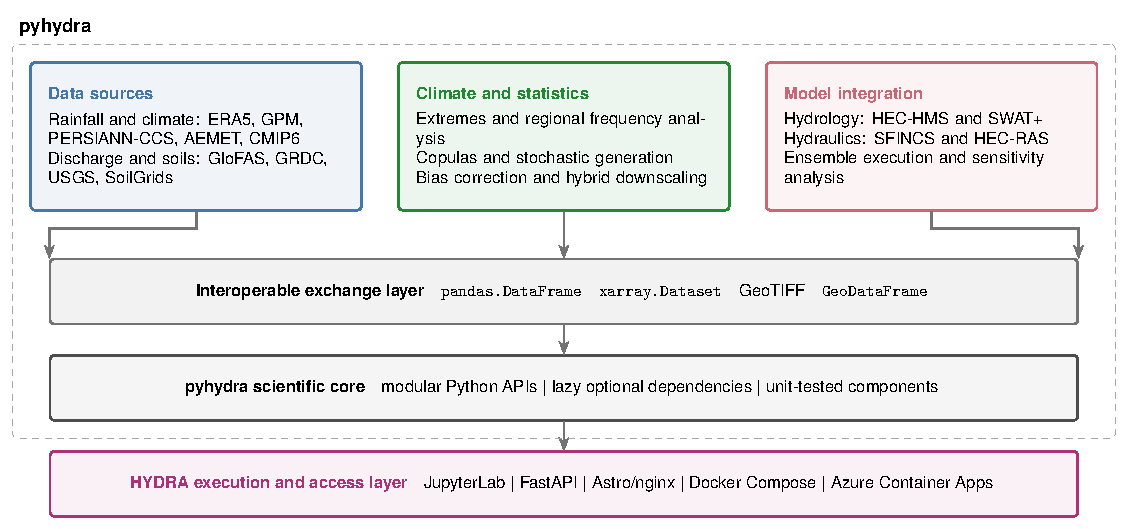
\includegraphics[width=\linewidth]{figures/fig01_architecture.pdf}
\caption{Software architecture. pyhydra provides four functional blocks of
reusable Python components connected through standard exchange formats;
HYDRA wraps the scientific core with reproducible execution, service and
access layers. Colours identify functional roles and do not encode values.
ChatGPT and Codex (OpenAI) assisted in writing the TikZ/Python code for
this diagram; the authors independently verified the scientific content,
edited the source and rendered the final figure.}
\label{fig:architecture}
\end{figure}

\begin{sloppypar}
Each pyhydra sub-module exposes its public API through its
\texttt{\_\_init\_\_.py}, so the import pattern is always
\texttt{from pyhydra.\allowbreak<block>.\allowbreak<module> import
<name>}. Optional heavy dependencies (PyMC, GDAL, GeoPandas, pyvinecopulib) are
imported lazily inside the functions that need them, so
the package loads -- and the parts of the API that do not need them run --
even when those dependencies are absent; a user who only needs
extreme-value analysis or bias correction can install pyhydra with
\texttt{pip} alone. Everything else is grouped into three installable
extras -- \texttt{statistics} (PyMC, pyvinecopulib, lmoments3),
\texttt{geospatial} (GeoPandas, rasterio, pykrige, earthaccess,
hydromt\_sfincs) and \texttt{models} (hecdss, pySWATPlus, spotpy,
NEOPRENE), plus a legacy \texttt{geo} extra for bare GDAL bindings and an
\texttt{all} extra covering all four -- so
\texttt{pip install "pyhydra[statistics]"} installs exactly what a given
workflow needs. One extended dependency, CoSMoS\_py (spatial random
fields), is not yet published on PyPI and must be installed separately
from its own repository. HYDRA's Docker Compose stack adds the extended
scientific dependencies and orchestrates a JupyterLab container, a FastAPI
backend and an nginx-served Astro frontend, built and deployed to Azure
Container Apps by a GitHub Actions workflow, with project data mounted from
a persistent file share rather than baked into the images.
\end{sloppypar}

\subsection{Software functionalities}
\label{sec:functionalities}

\cref{tab:modules} lists the fifteen sub-modules and their main
capabilities. The statistical modules implement established methodology
rather than novel formulations: bias correction follows standard
delta/quantile-mapping approaches \citep{teutschbein2012biascorrection},
regional frequency analysis follows the index-flood/L-moments framework
\citep{hosking1997rfa}, and dependence modelling follows standard copula
theory \citep{genest2007copulas} -- consistent with the framing in
\cref{sec:motivation} that the contribution is architectural, not a new
statistical method.

\begin{table}[h]
\small
\centering
\caption{pyhydra modules by functional block.}
\label{tab:modules}
\begin{tabular}{@{}p{0.38\textwidth}p{0.12\textwidth}p{0.435\textwidth}@{}}
\toprule
Module & Block & Main capability \\
\midrule
\path{data_sources.rainfall} & Data & ERA5, GPM, PERSIANN-CCS, AEMET, OGIMET, Meteostat \\
\path{data_sources.river_discharge} & Data & GloFAS, GRDC, USGS \\
\path{data_sources.climate_change} & Data & CMIP6 via CDS and ESGF \\
\path{data_sources.soils} & Data & SoilGrids download \& USDA texture classification \\
\path{climate.time_series} & Climate & Event extraction, GEV/GPD fitting, NSE/KGE/PBIAS \\
\path{climate.spatial_analysis} & Climate & Regional frequency analysis, Gaussian/vine copulas, IDW/kriging/GP interpolation \\
\path{climate.stochastic_generation} & Climate & NEOPRENE (point NSRP, spatial STNSRP), CoSMoS random fields \\
\path{climate.bias_correction} & Climate & Delta method, empirical/quantile-delta/scaled-distribution mapping \\
\path{climate.hybrid_downscaling} & Climate & Hydrograph classification, MaxDiss selection, k-NN/RBF flood-map reconstruction \\
\path{modeling.hydrology.hec_hms} & Modelling & Project generation, DSS I/O, SCE-UA calibration via spotpy \\
\path{modeling.hydrology.swat} & Modelling & SWAT+ input generation, execution, output parsing \\
\path{modeling.hydraulic.sfincs} & Modelling & Model setup, boundary conditions, batch execution \\
\path{modeling.hydraulic.hec_ras} & Modelling & 1D/2D project automation, DSS result extraction \\
\path{modeling.hydraulic.sensitivity} & Modelling & Manning Monte Carlo ensembles, spatial impact regression \\
\path{uq} & UQ & Pilot-based emulability diagnostic, MaxDiss design, reduce-and-emulate vs.\ Monte Carlo \\
\bottomrule
\end{tabular}

\vspace{2pt}
{\footnotesize\emph{Abbreviations:} GEV/GPD, Generalised Extreme Value /
Generalised Pareto Distribution; NSE/KGE/PBIAS, Nash--Sutcliffe Efficiency /
Kling--Gupta Efficiency / Percent Bias; IDW, Inverse Distance Weighting;
GP, Gaussian Process; DSS, Data Storage System (HEC file format); SCE-UA,
Shuffled Complex Evolution -- University of Arizona; RBF, Radial Basis
Function.}
\end{table}
\FloatBarrier

Four design principles guide the implementation: \emph{modularity} (each
block can be used independently -- extreme-value analysis does not require
geospatial or modelling dependencies); \emph{reproducibility} (standardised
notebooks, explicit parameters and data conventions preserve the evidence
needed to regenerate a result, while identifying any required credentials,
input projects or host-installed engines);
\emph{interoperability} (NetCDF/\texttt{xarray}, GeoTIFF, \texttt{pandas}
and GeoJSON/\texttt{geopandas} as the common data currency between blocks
and with external tools such as QGIS); and \emph{operational transfer}
(documentation, example notebooks and a reproducible Docker environment are
treated as first-class deliverables, not optional accessories). A
\texttt{pytest} suite of 291 tests across seventeen modules exercises the
statistical, modelling and UQ utilities most exposed to regression. A GitHub
Actions workflow (Ubuntu, core plus lightweight extended dependencies
including PyMC) runs this suite on every push across a Python 3.9--3.12
matrix; the one test that depends on PyMC/pytensor is still marked
\texttt{optional\_dependency} and guarded to skip rather than fail if that
stack is unavailable or, as happens with the older PyMC resolved on Python
3.9, incompatible with the installed NumPy. For the code version in
Table~\ref{tab:metadata} (commit \texttt{5552aa9}, 4 August 2026), this
workflow reports 291/291 passed on Python 3.10--3.12 and 290 passed
plus 1 skipped on 3.9, with 30--31\% line coverage -- concentrated in the
statistical and modelling-adapter code exercised directly by unit tests,
lower in the data-connector and engine-automation modules whose
behaviour is instead exercised, not formally verified, by the pilot-case
notebooks of \cref{sec:examples} against real services and engines. Runs
archived at
\url{https://github.com/navass11/pyhydra/actions/runs/30904958268}.

\paragraph{Reproducibility boundary} Reproducibility is reported at the
level supported by each workflow. Extreme-value fitting, copula analysis
and bias-correction examples are executable from included or synthetic data
in the container. Public-data downloads are repeatable after the user
supplies the corresponding service credentials and records the query
metadata. HEC-HMS, HEC-RAS, SFINCS and SWAT+ workflows additionally require
the relevant engine and a model project; large pilot cases may also contain
third-party data that cannot be redistributed. HYDRA preserves notebooks,
parameters, adapters and standard outputs for these conditioned workflows,
but does not claim that containerising the Python layer redistributes
proprietary executables or restricted datasets.

\begin{figure}[h]
\centering
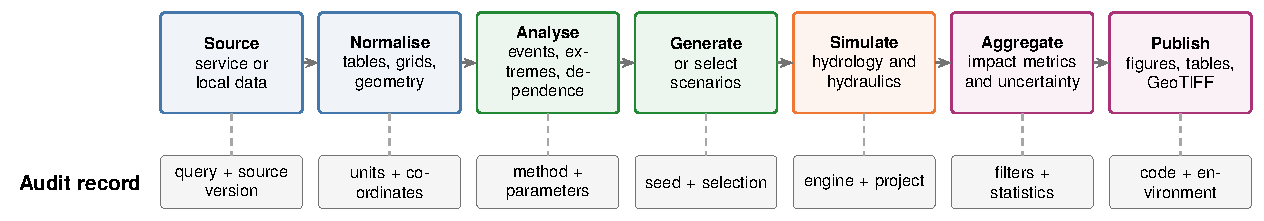
\includegraphics[width=\linewidth]{figures/fig02_reproducibility.pdf}
\caption{Reproducible workflow contract. Each transformation produces a
scientific artefact and an audit record sufficient to identify its source,
parameters, stochastic seed, external-engine configuration and software
environment. Colours identify functional stages and do not encode values.
ChatGPT and Codex (OpenAI) assisted in writing the TikZ/Python code for
this diagram; the authors independently verified the scientific content,
edited the source and rendered the final figure.}
\label{fig:reproducibility}
\end{figure}

\begin{sloppypar}
\paragraph{Uncertainty propagation and analysis} Rather than being confined
to a single module, uncertainty quantification cuts across the four
functional blocks: asymptotic, bootstrap and Bayesian posterior estimates on
extreme-value parameters and return levels
(\texttt{climate.time\_series}); posterior propagation across pooled
stations and prediction variance from spatial interpolators
(\texttt{climate.spatial\_analysis}); and Monte Carlo roughness ensembles
aggregated into spatial impact statistics with outlier screening
(\texttt{modeling.hydraulic}) -- the machinery exercised by the
SFINCS--HEC-RAS demonstration case in \cref{sec:examples}. The \texttt{uq}
module is a dedicated decision layer sitting above these: given an ensemble
and an expensive solver, it draws a nested maximum-dissimilarity pilot
charged against a fixed evaluation budget \texttt{n\_max}, measures that
pilot's cross-validated emulability against a declared family of cheap
emulators, and from that measurement chooses between completing a
reduce-and-emulate design or falling back to direct Monte Carlo -- rather
than fixing the choice by convention. A \texttt{StrategyDecision.margin}
flags choices taken on a hair's breadth, and a companion sequential-design
routine classifies each additional design point as improving, converged or
deteriorating so that a flattened error curve is not mistaken for one that
has turned upward.
\end{sloppypar}

\subsection{Sample code snippets}
\label{sec:snippets}

The snippet below chains three independent pyhydra components -- bias
correction, stochastic rainfall generation and bivariate copula analysis --
each usable on its own:

\begin{lstlisting}
from pyhydra.climate.bias_correction import BiasCorrection
from pyhydra.climate.stochastic_generation.point import NSRPModel
from pyhydra.climate.spatial_analysis.copulas import BivariateCopula

# 1. Bias-correct a regional climate model precipitation series
corrected = BiasCorrection.fit_transform(
    obs, hist, future, var='pr', method='qdm')

# 2. Calibrate and simulate a Neyman-Scott rectangular-pulse
#    stochastic rainfall generator (NEOPRENE)
model = NSRPModel(seasonality='monthly')
model.fit(observed_series)
synthetic = model.simulate(year_ini=2000, year_fin=2100)

# 3. Joint return period of a compound rainfall-discharge event
copula = BivariateCopula(family='gumbel').fit(rain_max, discharge_max)
x_or, y_or = copula.joint_return_period(t=100, kind='or')
\end{lstlisting}

%% ===========================================================================
\section{Illustrative examples}
\label{sec:examples}

pyhydra has been exercised through four flood-risk workflows at three
Spanish pilot sites, each reproduced as a notebook sequence under
\texttt{notebooks/\allowbreak pilot\_cases/} in the pyhydra repository itself
(\cref{tab:metadata}, C7); the companion HYDRA platform additionally
exposes the same notebooks through a browser, without requiring the
underlying pyhydra sequence to change. \cref{tab:reproducibility} traces
each workflow to its permanent notebook sequence and states, per the
reproducibility boundary defined above, what is required to re-run it.

\begin{table}[h]
\small
\centering
\caption{Traceability of the four illustrative workflows. Notebook paths
are relative to
\url{https://github.com/navass11/pyhydra/tree/v0.2.0/notebooks/pilot_cases/}.
``Open data'' marks inputs redistributable in full; ``Partial'' marks
cases where only some inputs (e.g.\ literature-based parameter
distributions or published aggregates) are open and the remainder is
project-specific and not redistributed here.}
\label{tab:reproducibility}
\setlength{\tabcolsep}{3pt}
\begin{tabular}{@{}p{0.11\textwidth}p{0.18\textwidth}p{0.14\textwidth}p{0.12\textwidth}p{0.28\textwidth}@{}}
\toprule
Case & Path & Open data & External engine & Reproduction \\
\midrule
Besaya &
\texttt{los\_\allowbreak corrales\_\allowbreak buelna/} (9 nb.$^{\ast}$) &
Partial & HEC-HMS, HEC-RAS & Conditioned on engine + project data \\[4pt]
M-30 Manzanares &
\texttt{m30\_\allowbreak manzanares/} (6 nb.) &
Partial & HEC-HMS, HEC-RAS & Conditioned on engine + project data \\[4pt]
Valencia DANA &
\texttt{valencia\_\allowbreak dana/} (2 nb.) &
Yes (AEMET, via \texttt{pyhydra-\allowbreak get-\allowbreak data}) & None &
Open and reproducible for the single-station and pooled-regional
analyses \\[4pt]
{\fontsize{9}{10}\selectfont SFINCS--HEC-RAS} &
\texttt{manning\_\allowbreak rugosidades/} (7 nb.) &
Partial (Manning distributions open; terrain/mesh project-specific) &
SFINCS, HEC-RAS & Conditioned on engine + project data \\
\bottomrule
\end{tabular}

\vspace{2pt}
{\footnotesize $^{\ast}$Eight sequential steps (01--06, 08); step 07 has two
notebook variants (\texttt{07\_hec\_ras\_hydraulics.ipynb}, the one
referenced by step 06 and used for the results reported here, and an
auxiliary \texttt{07\_hec\_ras\_hydraulics\_run.ipynb}).}
\end{table}

\textbf{Los Corrales de Buelna (Besaya River, Cantabria).} The founding
case of the methodology \citep{navas2018besaya}: 42 years of continuous
hydrological simulation (1970--2012) driven by 13 rain gauges, combined
with geostatistical event generation and k-NN probabilistic regression
($k=6$) to estimate return periods directly on flood impacts rather than on
design-storm discharge, in a valley-bottom town where more than 13\% of the
population lies within the mapped floodplain.

\textbf{M-30 Manzanares (Madrid).} Reproduces the multivariate flood
frequency methodology published by Navas et al. \citep{navas2024calle30}
(\cref{fig:m30}): 1{,}761 historical events from 17 rain gauges are
classified by PCA + k-means, an OpenTURNS Gaussian copula generates
approximately one million synthetic events over the resulting parameter space, MaxDiss
selects 1{,}000 representative events, which are simulated in HEC-HMS and
steady-state HEC-RAS 1D (303 cross-sections), and a k-NN regressor
reconstructs depths across the full synthetic ensemble under a compound
Poisson frequency model. The resulting $T{=}500$-year design depth at
Puente de Toledo exceeds the classical univariate-GEV estimate by 0.83~m
(7.61~m vs.\ 6.78~m), illustrating how neglecting inter-gauge dependence
can materially underestimate design hazard in a densely instrumented urban
catchment.

\begin{figure}[h]
\centering
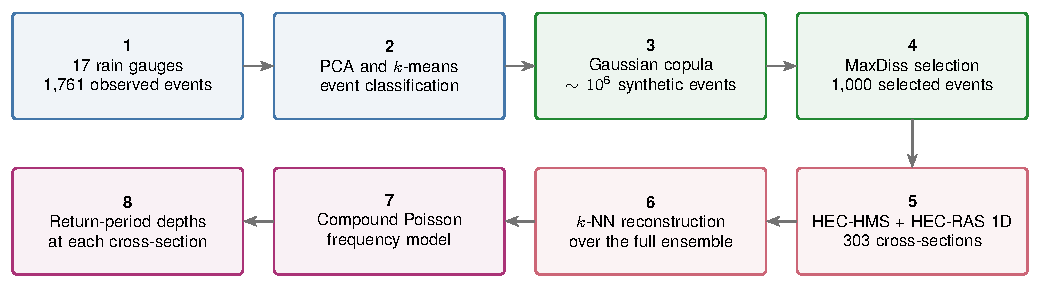
\includegraphics[width=\linewidth]{figures/fig04_m30_pipeline.pdf}
\caption{End-to-end pipeline reproduced in the M-30 Manzanares pilot case:
from 17 rain-gauge series (step 1) to return-period depths at two control
cross-sections, Puente de Toledo and Represa n\textordmasculine 9 (step 8),
following Navas et al. \citep{navas2024calle30}. Blue denotes observations and event
classification, green statistical generation and selection, orange physical
simulation and emulation, and purple frequency outputs. ChatGPT and Codex (OpenAI) assisted in writing the TikZ/Python code for
this diagram; the authors independently verified the scientific content,
edited the source and rendered the final figure.}
\label{fig:m30}
\end{figure}

\textbf{Valencia DANA (October 2024).} Implements an extreme-value fitting
comparison for the record-breaking rainfall event that struck the
Comunitat Valenciana on 29 October 2024, when AEMET's official post-event
report \citep{aemet2024dana} recorded new national single-station
intensity records at Turís (station 8337X); the dataset used here,
aggregated on calendar days, gives 710.8~mm/24h at that station. Two
notebooks, downloadable in full with \texttt{pyhydra-get-data
valencia\_dana} and requiring no AEMET credentials at run time, fit GEV
distributions at Turís with and without the event: single-station fits by
three methods (MLE, L-moments, Bayesian/MCMC), and a pooled-regional fit
(index-flood standardisation over all nine stations) by MLE and
L-moments. Including the event raises the estimated $T{=}100$-year return
level by a factor of 3.2--4.6 depending on method and scale, from
218--271~mm to 756--1{,}241~mm (\cref{fig:valencia}).

\begin{figure}[h]
\centering
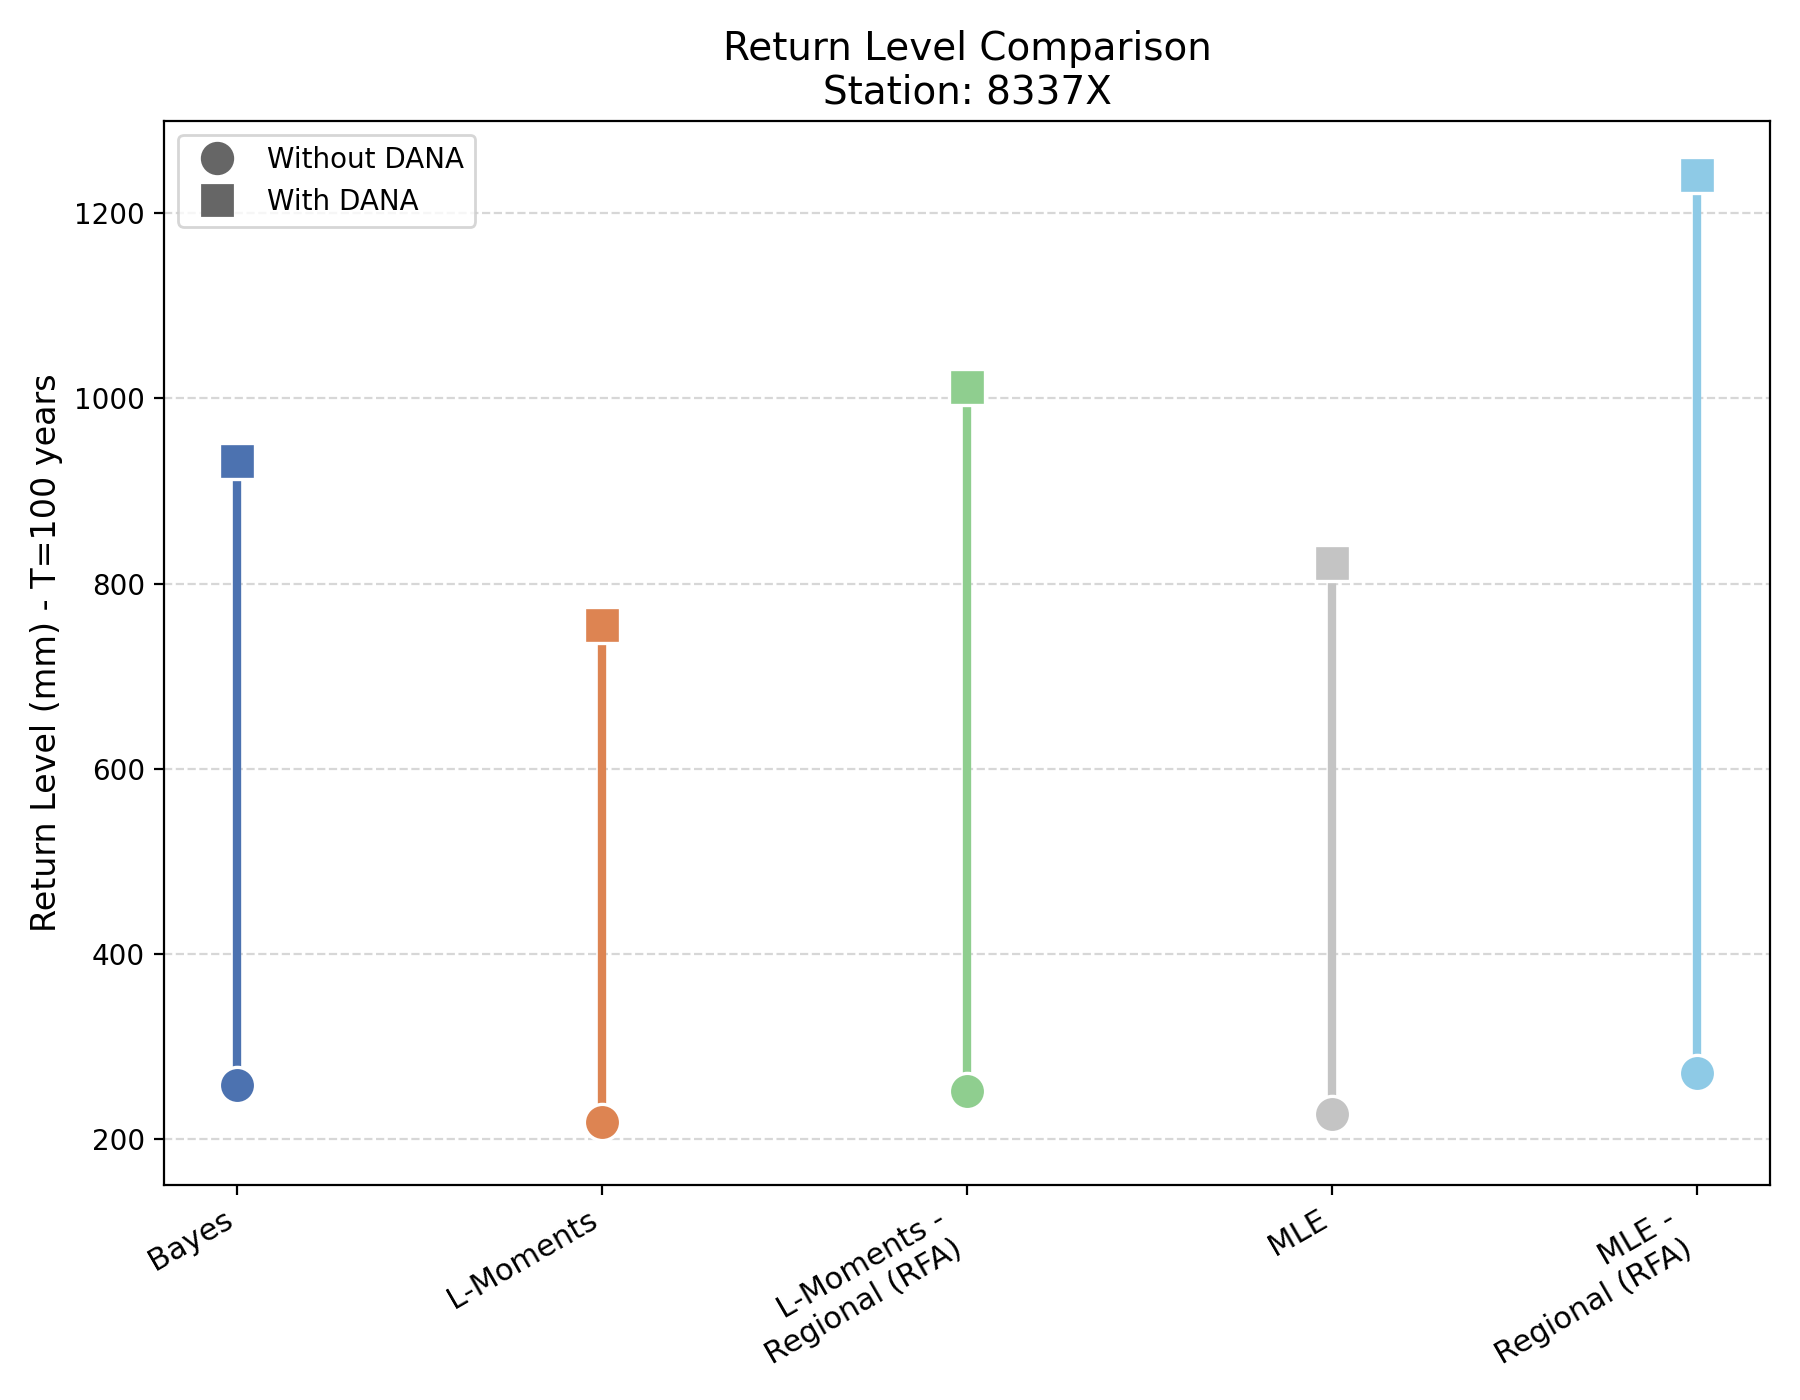
\includegraphics[width=0.85\linewidth]{figures/fig05_valencia_return_levels.png}
\caption{$T{=}100$-year return-level estimates at station 8337X (Turís),
with and without the 29 October 2024 event, for the single-station (MLE,
L-moments, Bayesian/MCMC) and pooled-regional-RFA (MLE, L-moments) fits
reproduced by the two archived notebooks described in the text.}
\label{fig:valencia}
\end{figure}

\begin{sloppypar}
\textbf{SFINCS--HEC-RAS uncertainty comparison (Besaya River).} A fourth
demonstration case exercises the uncertainty-propagation machinery of
\cref{sec:functionalities} across two independent 2D hydraulic engines:
\texttt{generate\_manning\_combinations} draws 1{,}000 Monte Carlo
roughness realisations over nine land-use classes from literature
distributions, the same ensemble is run through both SFINCS and HEC-RAS,
and \texttt{load\_sfincs\_ensemble}/\allowbreak
\texttt{load\_flood\_ensemble} together
with \texttt{spatial\_stats} and \texttt{manning\_flood\_regression}
aggregate each engine's inundation output into comparable spatial impact
statistics (\cref{fig:besaya-ensemble}). This section presents only the
pyhydra ensemble-generation and aggregation workflow, on one engine, as a
software demonstration; the resulting two-engine scientific comparison
between SFINCS and HEC-RAS is out of scope here and reported separately.
\end{sloppypar}

\begin{figure}[h]
\centering
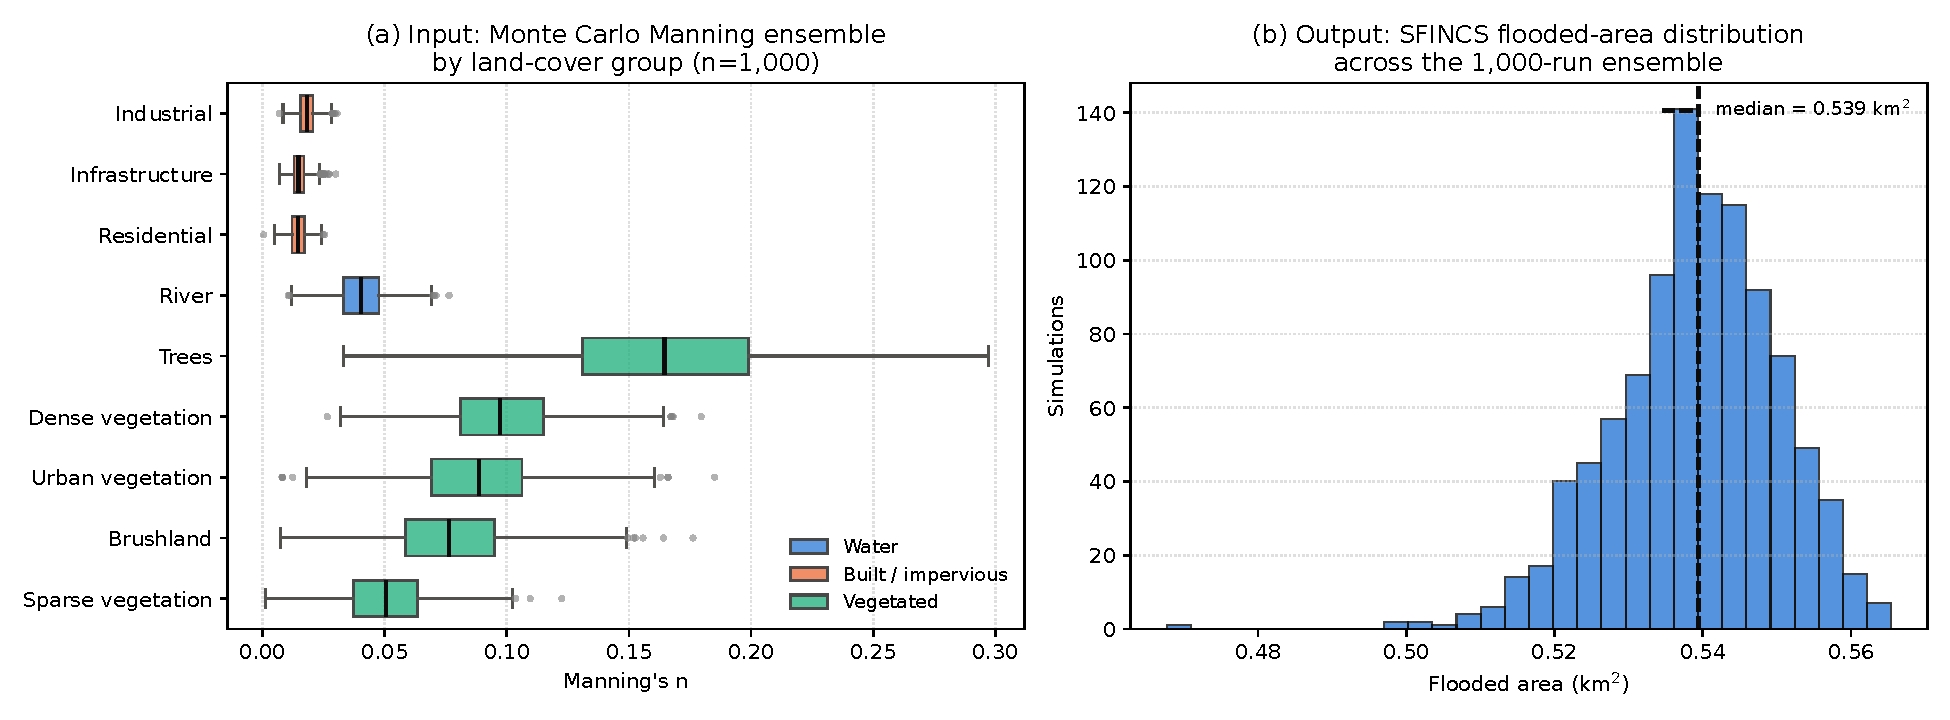
\includegraphics[width=\linewidth]{figures/fig03_besaya_ensemble.pdf}
\caption{(a) Input ensemble generated by pyhydra's
\texttt{generate\_manning\_combinations}: 1,000 Manning-roughness
combinations over nine land-use classes, grouped by land-cover type (water,
built/impervious, vegetated; boxes: interquartile range; line: median;
whiskers: non-outlier range; dots: outliers). (b) Output:
flooded-area distribution across the same 1,000-run SFINCS ensemble,
computed from the archived simulation outputs with pyhydra's
\texttt{load\_flood\_ensemble} and \texttt{flooded\_area}. This
single-engine distribution documents the ensemble-aggregation workflow
only; the two-engine SFINCS/HEC-RAS inundation comparison is out of scope
here and reported separately.}
\label{fig:besaya-ensemble}
\end{figure}

\begin{sloppypar}
The four workflows follow complementary execution paths -- continuous
impact-frequency analysis with hydraulic ensembles (Besaya), rainfall,
runoff and hydraulic modelling (M-30), and statistical inference without an
external solver (Valencia) -- and are not the only published applications
of the underlying methodology: the same building blocks also support
published work on Andean hydropower systems \citep{deljesus2020andinos}
and reservoir inflows under climate change \citep{navas2025simpce}.
\end{sloppypar}

%% ===========================================================================
\section{Impact}
\label{sec:impact}

pyhydra formalises, as versioned and tested software, a line of flood-risk
research that previously existed as independent, non-interoperable study
codebases. Five published journal articles and one journal article in
press, produced by the authors' group, already rely on methods now
consolidated in pyhydra
\citep{navas2018besaya,diezsierra2023neoprene,navas2024calle30,navas2025simpce,deljesus2020andinos,urrea2026vine}.
Conference proceedings and manuscripts still under review are not counted
here as impact evidence. This methodological track record predates pyhydra
as a software product and shows that the underlying methods work; it is
distinct from, and does not substitute for, evidence that the software
itself has been adopted outside the authors' group.

Beyond consolidating methods that already existed as separate scripts,
having them share a common ensemble and impact-statistics layer
(\cref{sec:functionalities}) also opens questions that were impractical to
pose across four disconnected codebases: how differently two hydraulic
engines propagate the same roughness ensemble into inundation extent, as
exercised in \cref{sec:examples}; and how directly conditioning
frequency analysis on spatial impacts, rather than on discharge or rainfall
alone, shifts design estimates relative to the classical univariate route,
as the M-30 comparison in \cref{sec:examples} begins to quantify.

As a software product, pyhydra's impact so far is internal to the authors'
group, reported as such rather than overstated. A new case study is now
assembled from existing, unit-tested building blocks rather than
rewritten -- what let the four workflows of \cref{sec:examples} share one
code base instead of four disconnected scripts, and what made the M-30
comparison against the classical univariate method (0.83~m higher
$T{=}500$-year depth) straightforward rather than a bespoke
re-implementation. Archiving pyhydra under the MIT license on Zenodo
\citep{navas2026pyhydra} gives each downstream publication a citable,
versioned code reference, closing a gap that affected the earlier,
unpublished study scripts. The companion HYDRA platform
(\cref{sec:architecture}), archived separately \citep{navas2026hydrarepo}
and reachable, as of 30 July 2026, at the URL given in its
README\footnote{Ephemeral Azure Container Apps deployment; useful for
evaluation but not a citable scholarly reference. The Zenodo records
remain the durable citation for both components.}, removes
local-environment setup as a barrier to inspecting any of the four
notebooks with the full scientific stack pre-installed.

Because the public GitHub release is recent, independent adoption metrics
-- downloads, external contributions, third-party citations, teaching or
commercial use -- are not yet available, and none are claimed here.
pyhydra is used in ongoing doctoral and project research at IHCantabria --
Universidad de Cantabria; broadening use beyond the authors' group is
future work (\cref{sec:conclusions}).

%% ===========================================================================
\section{Conclusions}
\label{sec:conclusions}

pyhydra turns a decade-long line of impact-based flood-risk research into
modular, tested, MIT-licensed software: an installable scientific core with
a modular, reproducible architecture; harmonised access to hydro-climatic
and hydrological data; automation of hydrological and hydraulic models; and
propagation and analysis of uncertainty across the whole chain. The
companion HYDRA platform separately provides an optional operational web,
API, Jupyter and Docker environment on top of this core, without changing
how pyhydra itself is installed or used. Four workflows at three
Spanish pilot sites -- Besaya, M-30 Manzanares and Valencia -- span fluvial,
urban and compound-event flood risk. Together they
show that the same modular components support markedly different study
designs, from continuous stochastic simulation to multivariate copula-based
frequency analysis and cross-engine Monte Carlo comparison. Ongoing work
focuses on widening automated test coverage as new modules are added,
adding adapters for further hydraulic/hydrological engines, and documenting
a stable public API to lower the barrier for external contributions beyond
the authors' own research group.

The present release also has explicit limits. Short records and rare
extremes remain information-limited even under bootstrap, Bayesian or
regional uncertainty quantification, and regional analysis still requires a
defensible homogeneous region; stochastic generators do not by themselves
resolve climate non-stationarity; emulators and MaxDiss selection reduce
hydraulic-ensemble cost but cannot replace physical-model validation, and
depend on the representativeness of the simulated subset; and
reproducibility of externally executed models is conditioned by engine
version, licences and project availability. HYDRA makes these dependencies
explicit and auditable rather than removing them.

%% ===========================================================================
\section*{CRediT authorship contribution statement}
\textbf{Salvador Navas:} Conceptualization, Methodology, Software, Data
curation, Formal analysis, Investigation, Validation, Visualization, Writing
-- original draft, Writing -- review \& editing. \textbf{Manuel del Jesus:}
Conceptualization, Methodology, Resources, Supervision, Funding acquisition,
Validation, Writing -- review \& editing.

\section*{Funding}
Manuel del Jesus acknowledges the support provided by Project PCI2024-153483
(WaMA-WaDiT, ``Water Management and Adaptation based on Watershed Digital
Twins''), funded by MICIU/AEI/10.13039/501100011033 and co-funded by the
European Union. This research did not receive any other specific grant from
funding agencies in the public, commercial or not-for-profit sectors. The
funding bodies had no role in study design, data collection, analysis,
interpretation, manuscript preparation or the decision to submit the article
for publication.

\section*{Declaration of competing interests}
The authors declare that they have no known competing financial interests or
personal relationships that could have appeared to influence the work
reported in this paper.

\section*{Data availability}
The pyhydra version described in this article is available through the
versioned GitHub and Zenodo records in Table~\ref{tab:metadata}. The
companion HYDRA deployment platform used to run the browser-accessible
workflows in \cref{sec:examples} is likewise open source and MIT-licensed,
and is archived separately \citep{navas2026hydrarepo}. The pilot workflows
additionally consume public third-party data services cited in the text.
Proprietary hydraulic-engine projects and restricted project datasets
cannot be redistributed; their absence does not prevent inspection or reuse
of the open statistical components, interfaces and example workflows.

\section*{Declaration of generative AI and AI-assisted technologies in the
manuscript preparation process}
During manuscript preparation (2026), the authors used ChatGPT and the
Codex coding assistant (OpenAI; specific model versions not recorded) to
assist with language editing, text revision, manuscript formatting and
the drafting of figure code (identified in the affected captions); during
these revisions (30 July -- 4 August 2026), Claude Sonnet 5 (model ID
\texttt{claude-sonnet-5}, Anthropic) assisted with editing manuscript
text, diagnosing and fixing software defects surfaced by the
continuous-integration workflow added in \cref{sec:functionalities}, and
re-executing the Valencia notebooks to regenerate \cref{fig:valencia}
from their output. In all cases, assistance was limited to code and
text; it did not extend to designing the underlying methodology or
validating its scientific content. After using these tools, the authors
reviewed and edited the content and code as needed, checked the cited
evidence and numerical values, and take full responsibility for the
content of the published article and the archived code.

\section*{Acknowledgements}
The stochastic-impact methodology consolidated in this software originates
from doctoral and research work carried out at IHCantabria -- Instituto de
Hidr\'aulica Ambiental de la Universidad de Cantabria. The authors thank the
Confederaci\'on Hidrogr\'afica del Cant\'abrico and the Agencia Estatal de
Meteorolog\'ia for hydrological and climate records used in the associated
case studies, and the Instituto Geogr\'afico Nacional for openly available
PNOA products. Computationally intensive workflows used IHCantabria
infrastructure and resources provided by the University of Cantabria through
its Microsoft Azure academic subscription.

%% ===========================================================================
\bibliographystyle{elsarticle-num}
\bibliography{references}

\section*{Current executable software version}
pyhydra v0.2.0 (commit \texttt{5552aa9}) is the executable software version
described in this publication; its archived record and immutable GitHub
tag link are provided in Table~\ref{tab:metadata} and should be cited
independently using the corresponding Zenodo record
\citep{navas2026pyhydra}. The companion HYDRA deployment platform used for
the browser-accessible examples in \cref{sec:examples} is archived
separately at v0.1.2 (commit \texttt{627a838}) \citep{navas2026hydrarepo}.

\end{document}
